\documentclass[14pt]{article}

\usepackage{graphicx}


\usepackage{lipsum}

\usepackage{mathtools}

\usepackage[margin = 1in]{geometry}

\usepackage{amssymb}
\usepackage{amsmath}

\usepackage{caption}
\usepackage{subcaption}

\usepackage[nottoc,numbib]{tocbibind}

\usepackage[perpage, bottom]{footmisc}
\renewcommand{\thefootnote}{\fnsymbol{footnote}}
%\footnote[number]{text}
%1 asterisk *
%2 dagger †
%3 double dagger ‡
%4 section symbol §
%5 paragraph ¶
%6 parallel lines ‖
%7 two asterisks **
%8 two daggers ††
%9 two double daggers ‡‡


% NOTE: put footmisc hyperref and footnotebackref in this order, this way the footnote hyperlinks will lead to the footnote and not the title page
\usepackage{url}
\usepackage{hyperref}
\hypersetup{colorlinks = true, citecolor = blue, linkcolor = blue, urlcolor = blue}

\usepackage{footnotebackref}

% to place figures in the section they are meant for
\usepackage[section, above, below]{placeins}



% Using titlepage Environment instead of \maketitle
% \title{Visualizing functions using Python and Octave}
% \author{Atharva Aalok}
% \date{July 9, 2021}



\begin{document}
    \begin{titlepage}
        \begin{center}
            \rule{\textwidth}{1pt}\\
            \Huge
            \textbf{Using \\ Linear Regression \\ to fit models to Data }\\
            \rule{\textwidth}{1pt}
            \vfill
            
            \Large
            \textbf{Submitted by:}
            \medskip

            Atharva Aalok
            \vfill

            
\includegraphics[width = 2in]{Images/IITM_logo.svg.png}
            \vfill

            Department of Aerospace Engineering,
            \medskip

            Indian Institute of Technology Madras
            \vfill

            July 14, 2021

        \end{center}
    \end{titlepage}


    \renewcommand*\contentsname{\huge Summary}
    \large
    \tableofcontents
    \normalsize


    \pagebreak
    \huge
    \section{Introduction}
    \normalsize
    Linear Regression is a technique using which we can fit models to data which are linear with respect to the parameters used.

    Let us say we have some variable y which depends on an independent variable x.
    We want to fit a model which can predict y given x.
    The process of Linear Regression requires us to assume a model to fit to the data.
    Here we choose the model y = mx + c.

    We may not be able to fit the data perfectly for each data point but we try to fit the data as closely as possible.
    To do this we define a measure of error in our model.
    Specifically we choose the sum of squares of error in predicting y for each data point as our Cost(Error) function. We denote the cost function by J. We will also refer to our data points as training examples.

    Our task then is to choose parameters m and c so as to minimize our cost function J. Hence we have the following problem to solve: If we have n training examples then our error on each training example is given by $ \epsilon_{i} $ as

    \begin{align}
        \epsilon_{1} &= mx_{1} + c - y_{1} \\
        \epsilon_{2} &= mx_{2} + c - y_{2} \\
        &\vdotswithin{=} \nonumber \\
        \epsilon_{n} &= mx_{n} + c - y_{n} \\
    \end{align}

    \noindent and our cost function is which is a function of parameters m and c is given by,
    \[ J(m,c) = \sum_{i=1}^{n} \epsilon_{i}^2 \]

    \noindent We can write all this succinctly using vector notation as

    % NOTE: matrix environment has to be put in between $$
    \[
    \begin{bmatrix}
        \epsilon_{1}\\
        \epsilon_{2}\\
        \vdots\\
        \epsilon_{n}
    \end{bmatrix}
    =
    \begin{bmatrix}
        y_{1}\\
        y_{2}\\
        \vdots\\
        y_{n}
    \end{bmatrix}
    -
    \begin{bmatrix}
        1 & x_{1}\\
        1 & x_{2}\\
        \vdots\\
        1 & x_{n}
    \end{bmatrix}
    \begin{bmatrix}
        c\\
        m
    \end{bmatrix}
    \]

    \noindent We denote the vector of epsilons by $ \vec{\epsilon} $ the vector of c and m by $ \vec{v} $ the vector of $ y_{i}'s $ by $ \vec{y} $ and the matrix multiplying $ \vec{v} $ by $ \textbf{A} $.

    \noindent We want to minimize:
    $ \left\lVert \vec{\epsilon} \right\rVert $


    \noindent It can be shown using calculus that the parameter vector that minimizes our error function is given By
    \[ \vec{v} = (\textbf{A}^{T} \textbf{A})^{-1} \textbf{A}^{T} \vec{y} \]


    Using the above approach we have tried to fit a model of the form y = mx + c to our 3 datasets and analyze whether such a model is a good choice for our data \footnote[2]{Find the Datasets here - \url{GITHUB}}.




    %\pagebreak
    \huge
    \section{Applying Linear Regression}
    \normalsize
    We perform linear regression on our 3 data sets. To analyze whether a model of the form y = mx + c is a good approximation we divide each dataset into 3 subsets. We perform linear regression using 50, 100 and 200 training examples of each data set.\footnote[8]{For the MATLAB codes for linear regression refer - \url{GITHUB}}

    % NOTE: I put \\ as a smart move to make the table appear after this line
    \noindent The values we obtained are: \\

    \begin{table}[hbt!]
        \centering
        \begin{subtable}{.5\textwidth}
        \centering
            \begin{tabular}{|l|l|l|}
                \hline
                DataSetSize & m & c \\
                \hline 
                50 & 2.011 & 1.188 \\ 
                \hline
                100 & 2.008 & 1.266 \\ 
                \hline
                200 & 2.006 & 1.377 \\  
                \hline
            \end{tabular}
        \caption{Data Set 1}
        \label{tbl:ParamsD1}
        \end{subtable}
        ~
        \begin{subtable}{.5\textwidth}
        \centering
            \begin{tabular}{|l|l|l|}
                \hline
                DataSetSize & m & c \\
                \hline 
                50 & 2.011 & 1.196 \\ 
                \hline
                100 & 2.008 & 1.272 \\ 
                \hline
                200 & 2.006 & 1.381 \\  
                \hline 
            \end{tabular}
        \caption{Data Set 2}
        \label{tbl:ParamsD2}
        \end{subtable}
        ~
        \begin{subtable}{.5\textwidth}
        \centering
            \begin{tabular}{|l|l|l|}
                \hline
                DataSetSize & m & c \\
                \hline 
                50 & 2.000 & 1.005 \\ 
                \hline
                100 & 2.000 & 1.005 \\ 
                \hline
                200 & 2.000 & 1.005 \\ 
                \hline
            \end{tabular}
        \caption{Data Set 3}
        \label{tbl:ParamsD3}
        \end{subtable}

    \caption{Parameter Values obtained by Linear Regression}
    \label{tbl:ParamsData}
    \end{table}


    We observe that m and c remain almost constant as we vary number of training examples from 50 to 100 to 200. Hence a linear model is a good fit for our data.


    %\pagebreak
    \huge
    \section{Comparing Model with Real Data}
    \normalsize
    We plot the predictions that our model makes on the input x and also plot the real data points on top to compare the accuracy of our model visually.
    \begin{figure}[!h]
        \centering
        \begin{subfigure}{\textwidth}
            \centering
            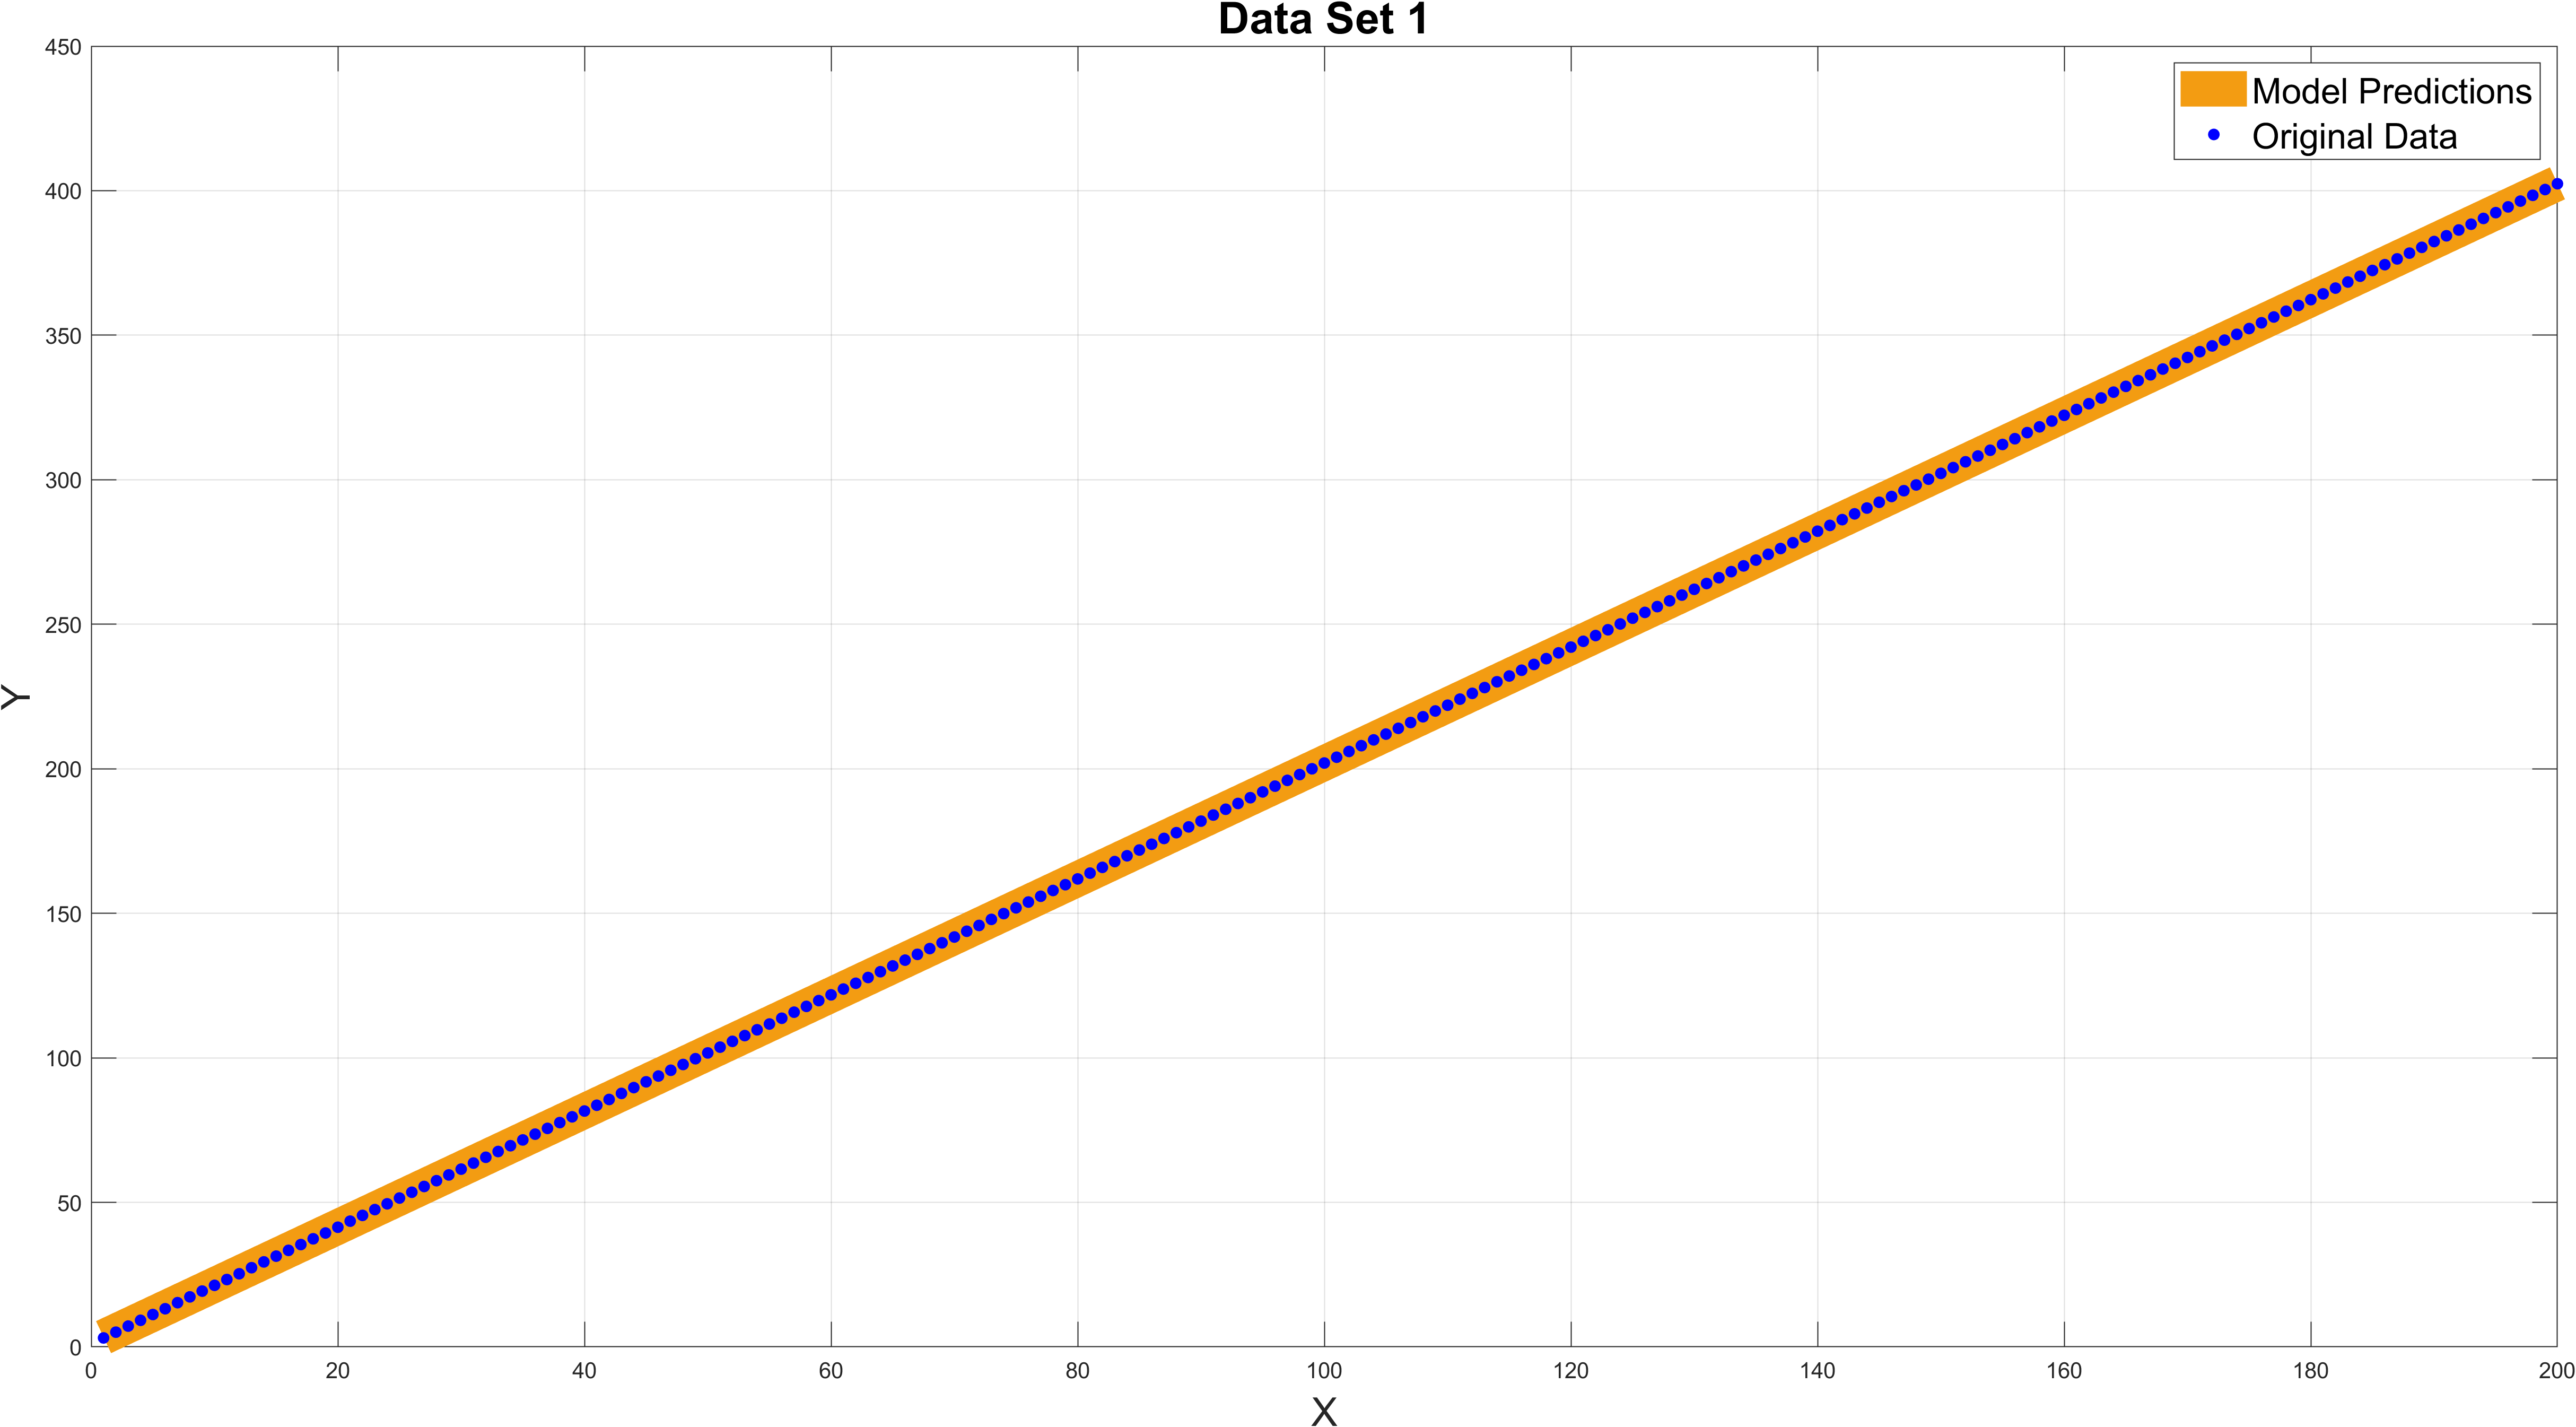
\includegraphics[width = \textwidth]{Images/Table_data1.png}
            \caption{Data Set 1}
        \end{subfigure}
        \begin{subfigure}{\textwidth}
            \centering
            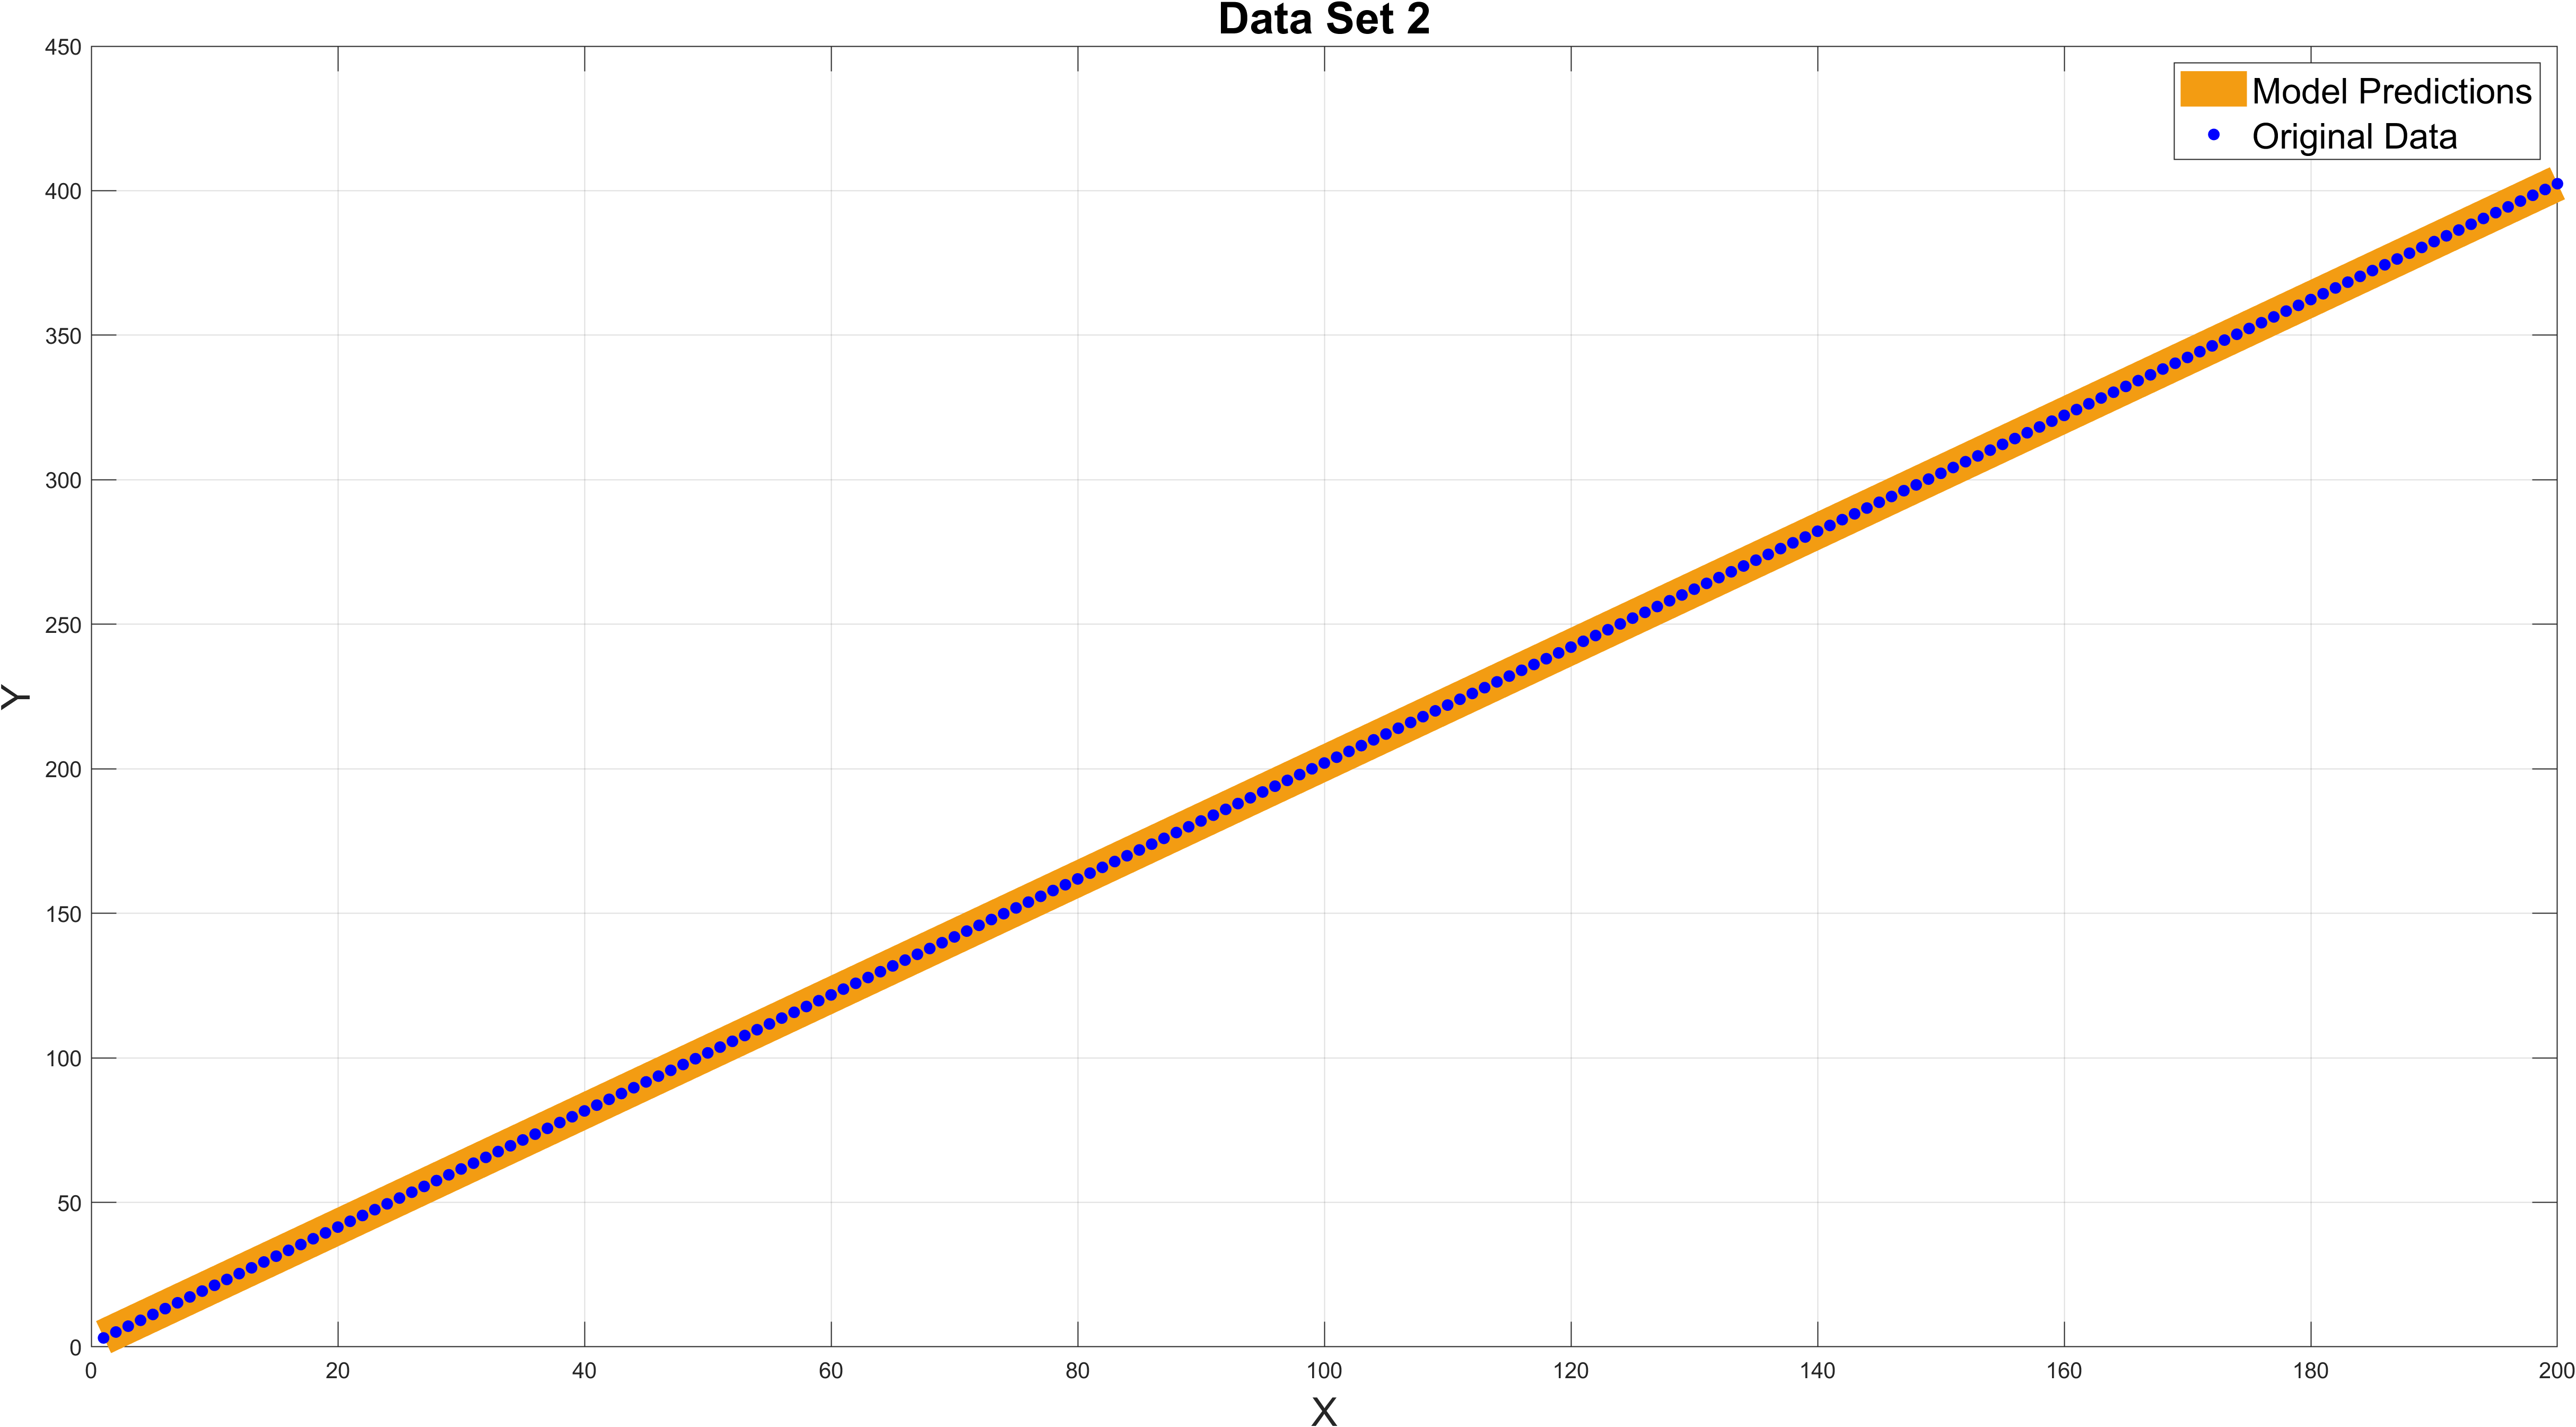
\includegraphics[width = \textwidth]{Images/Table_data2.png}
            \caption{Data Set 2}
        \end{subfigure}
        % \caption{Caption 1}
    \end{figure}
    \begin{figure}[h]\ContinuedFloat
        \begin{subfigure}{\textwidth}
            \centering
            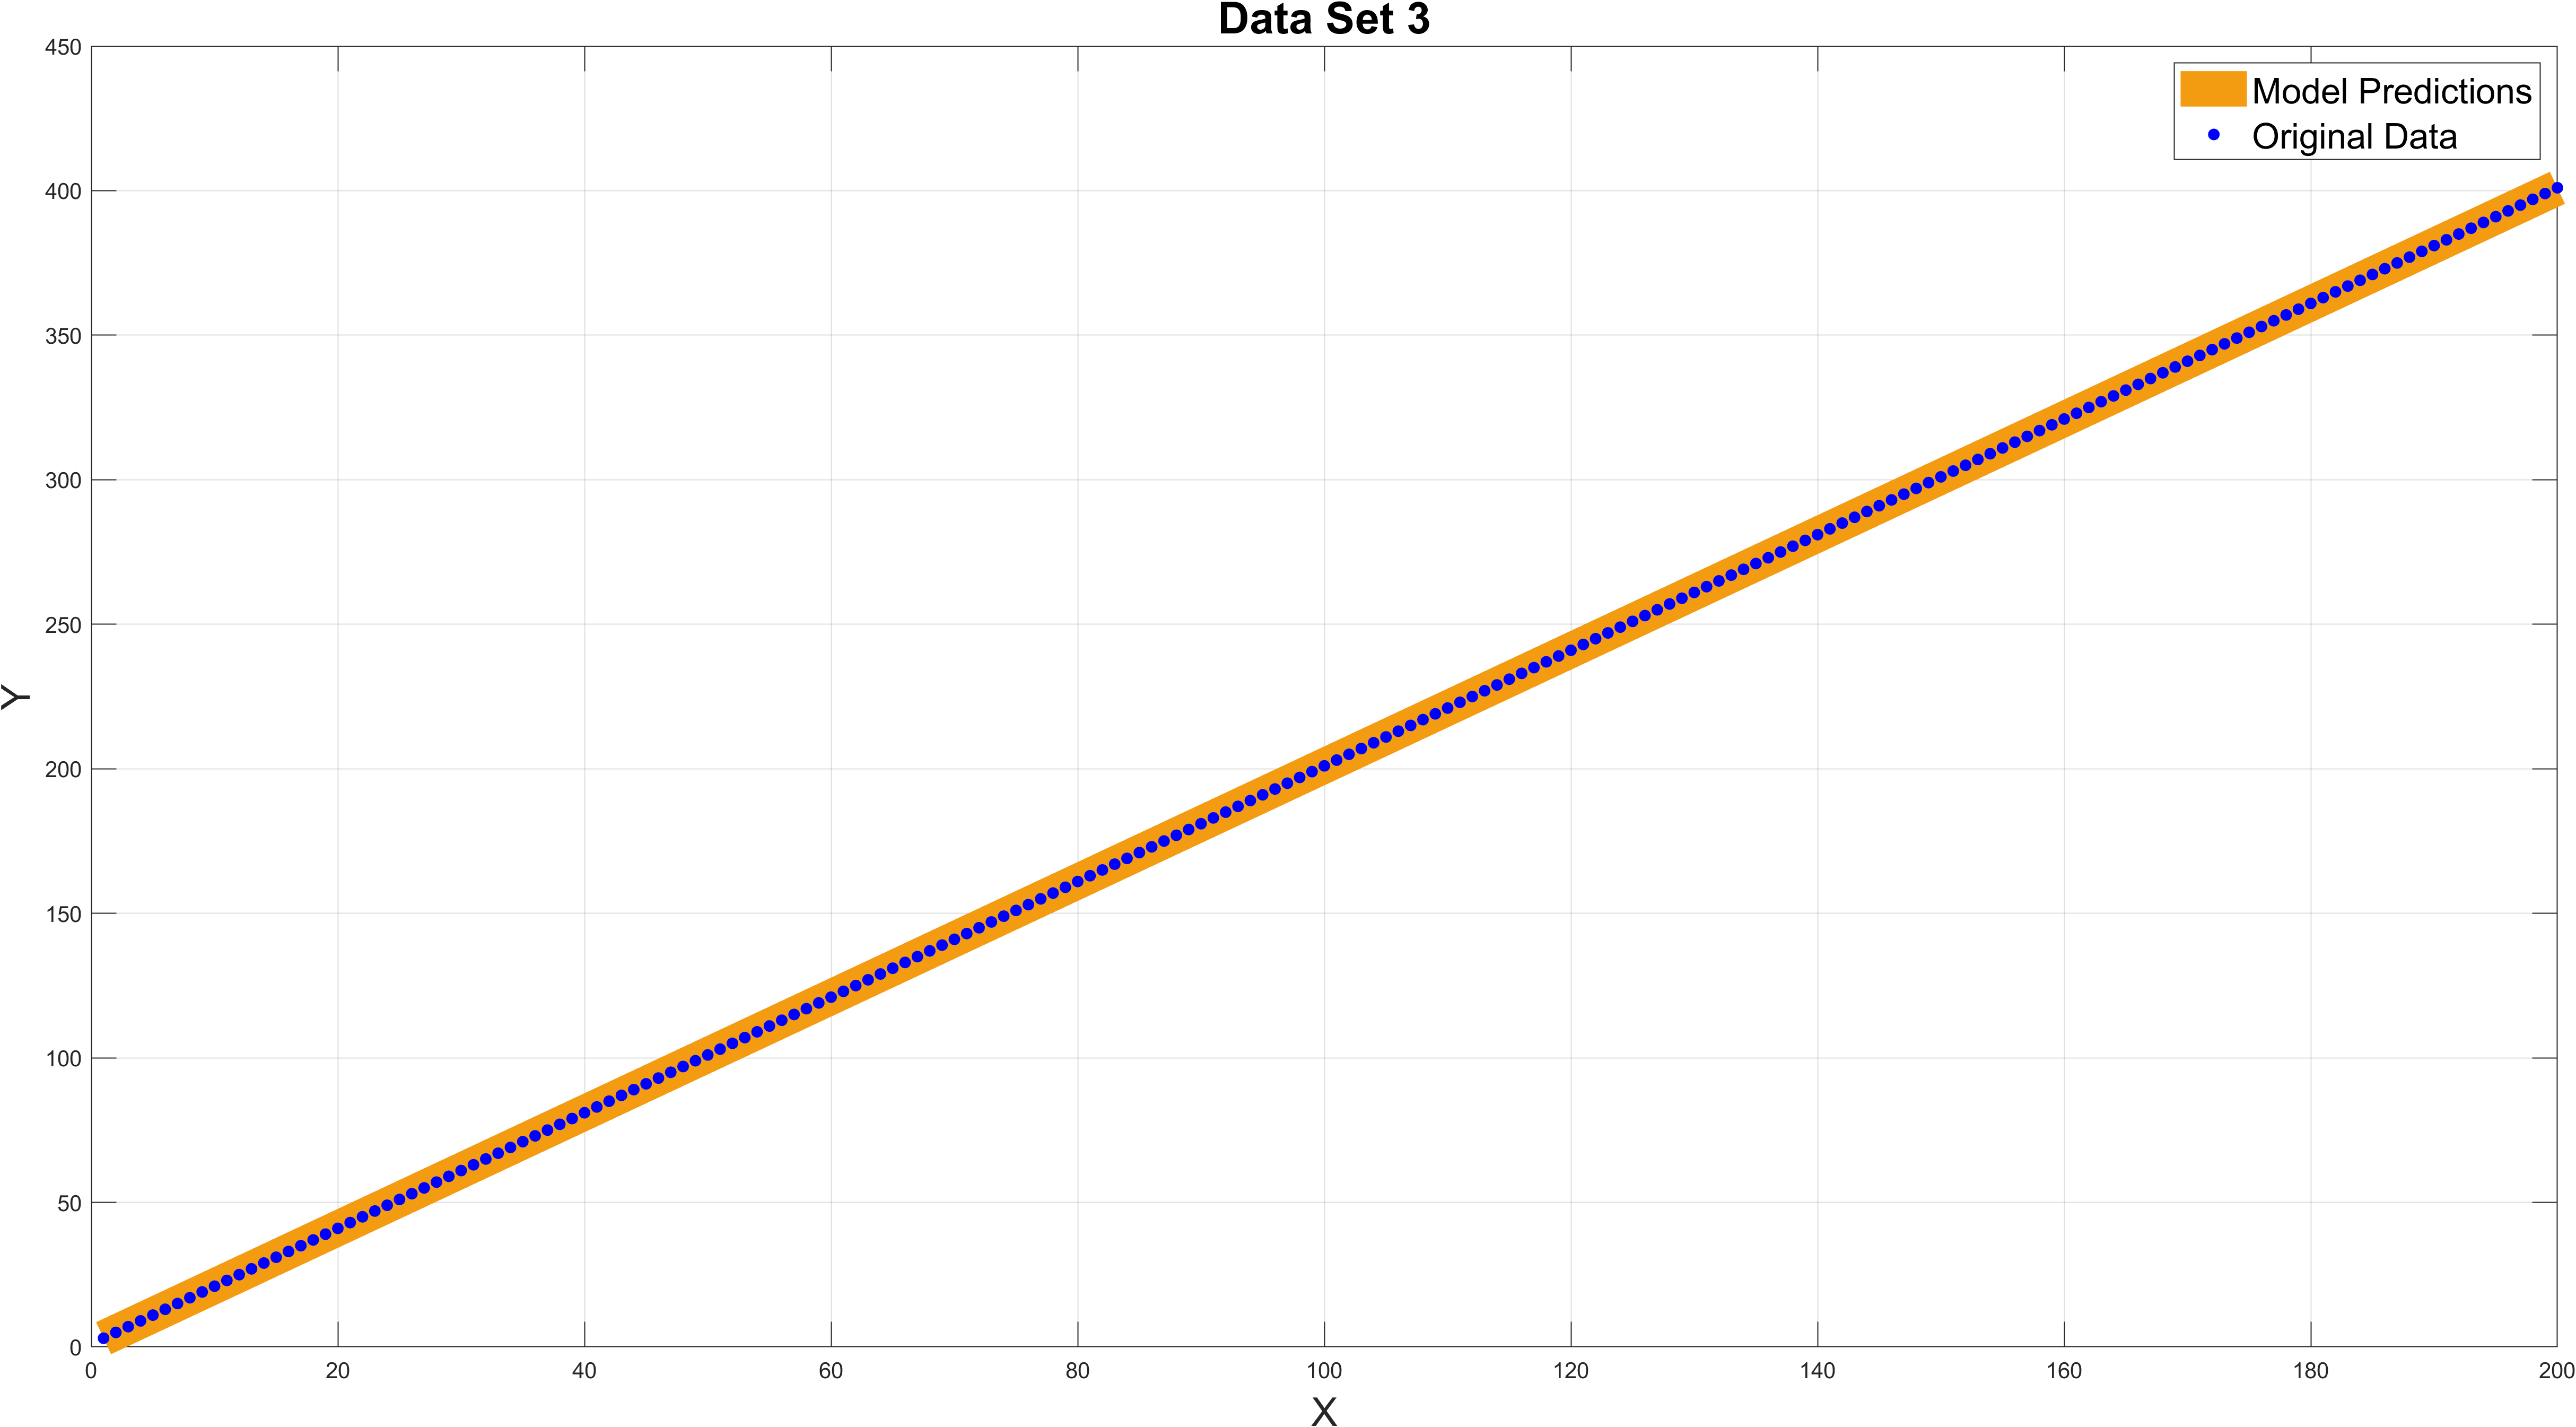
\includegraphics[width = \textwidth]{Images/Table_data3.png}
            \caption{Data Set 3}
        \end{subfigure}
        \caption{Models fitted using Linear Regression}
    \end{figure}


    \huge
    \section{Inferences}
    \normalsize
    We observe that m and c are almost constant for our data as we vary number of training examples from 50 to 100 to 200. Hence a linear model is a good fit for our data.
    Also it is visually clear that a linear model fits the original data distribution extremely well.

    Since the data agrees very well with our model we use this to make predictions for y.
    Hence we make predictions on y given x for the 3 data sets as:\\ \\
    \noindent Model predictions for Data Set 1:
    \[ y = 2.006x + 1.377 \]
    \noindent Model predictions for Data Set 2:
    \[ y = 2.006x + 1.381 \]
    \noindent Model predictions for Data Set 3:
    \[ y = 2.000x + 1.005 \]

    

    \pagebreak
    \nocite{*}
    \bibliographystyle{plain}
    \bibliography{biblio}

\end{document}